\documentclass[14pt]{article}
\usepackage{amsmath}
\usepackage{amssymb}
\usepackage{cancel}
\usepackage{graphicx}
\usepackage{geometry}
\usepackage[font=small,labelfont=bf]{caption} % Required for specifying captions to tables and figures
\geometry{
	a4paper,
	total={170mm,257mm},
	left=20mm,
	top=10mm,
}
\begin{document}
	\title{Calculus II and III Notes}
	\author{Saptarshi Dey}
	\date{March 14, 2021}
	\maketitle
	\section{Inverse Hyperbolic Trigonometric Functions}
	\large{Pre-requisites/Synopsis :-}
	\begin{equation}
		\sinh(x)=\frac{e^x-e^{-x}}{2}
	\end{equation}
	\begin{equation}
		\cosh(x)=\frac{e^x+e^{-x}}{2}
	\end{equation}
	\begin{equation}
		\tanh(x)=\frac{e^x-e^{-x}}{e^x+e^{-x}}
	\end{equation}
	Let's assume $\sinh^{-1}(x)=\ln|f(x)|$ where $f(x)$ is some function of $x$ 
	\\ \begin{equation*}
	\therefore \frac{e^{\ln|f(x)|}-e^{-\ln|f(x)|}}{2} = x	
	\end{equation*}
	\begin{equation*}					%Equation environment with * won't be numbered
	\implies f(x)-\frac{1}{f(x)} = 2x		
	\end{equation*}
	\begin{equation*}
	\implies f^2(x)-2xf(x)-1 = 0		
	\end{equation*}
	Solving this quadratic equation, we get,
	\begin{equation*}
		f(x)=x\pm\sqrt{1+x^2}
	\end{equation*}
	If $f(x)=x-\sqrt{1+x^2}$, then $f(x)<0$ for all $x\in(-\infty,0)$
	\\ But $f(x)$ can't be -ve since $\ln|f(x)|$ will be an complex number.
	$\therefore f(x)=x+\sqrt{1+x^2}$
	\begin{equation}
		\therefore \boxed{\sinh^{-1}(x)=\ln|x+\sqrt{1+x^2}|}
	\end{equation}
	Similarly, we can prove,
	\begin{equation}
	\boxed{\cosh^{-1}(x)=\ln|x+\sqrt{x^2-1}|}
	\end{equation}
	Let $\tanh^{-1}(x)=\ln|f(x)|$
	\begin{equation*}
		\therefore \frac{e^{\ln|f(x)|}-e^{-\ln|f(x)|}}{e^{\ln|f(x)|}+e^{-\ln|f(x)|}}=x
	\end{equation*}
	\begin{equation*}
	\implies \frac{f(x)-\frac{1}{f(x)}}{f(x)+\frac{1}{f(x)}}=x
	\end{equation*}
	Using componendo-dividendo,
	\begin{equation*}
	\frac{1}{f^2(x)}=\frac{1-x}{1+x}
	\end{equation*}
	\begin{equation*}
	\implies f(x)=\sqrt{\frac{1+x}{1-x}}
	\end{equation*}
	\begin{equation}
	\therefore \boxed{\tanh^{-1}(x)=\ln(\sqrt{\frac{1+x}{1-x}})=\frac{1}{2}\ln(\frac{1+x}{1-x})}
	\end{equation}
	\section{Basic Integration Problems}
	\subsection{Evaluate}
	1. $\displaystyle \int \frac{\sqrt{x^2+1}-\sqrt{x^2-1}}{\sqrt{x^4-1}}dx$ \\
	2. $\displaystyle \int \frac{x^2}{(x\sin x+\cos x)^2}dx$ \\
	3. $\displaystyle \int \frac{dx}{\sqrt[4]{(x-1)^3(x+2)^5}}$
	\subsection{Solutions}
	1. I = $\displaystyle \int\frac{\sqrt{x^2+1}-\sqrt{x^2-1}}{\sqrt{x^2-1}\sqrt{x^2+1}}dx$ \\ \\= $\displaystyle \int\frac{dx}{\sqrt{x^2-1}} - \int\frac{dx}{\sqrt{x^2+1}} = \boxed{\cosh^{-1}(x)-\sinh^{-1}(x)+C}$ \\ \\ \\
	2. I = $\displaystyle\int x \sec x \frac{x \cos x}{(x\sin x+\cos x)^2}dx$ \\
	$\displaystyle =x \sec x \int \frac{x \cos x}{(x\sin x+\cos x)^2}dx + \int \frac{\sec x+x\tan x}{x\sin x+\cos x}dx$ \\ \\
	$\displaystyle =-\frac{x\sec x}{x\sin x+\cos x}+\int\frac{(\sec x+x\tan x)\times\cos^2 x}{(x\sin x+\cos x)\times\cos^2 x}dx+C_1$ \\ \\
	$\displaystyle =-\frac{x\sec x}{x\sin x+\cos x}+\int\frac{\cancel{(x\sin x+\cos x)}}{\cancel{(x\sin x+\cos x)}\cos^2(x)}dx+C_1$ \\ \\
	$\displaystyle = \boxed{\tan x -\frac{x\sec x}{x\sin x+\cos x}+C}$ \\ \\ \\
	3. Let $a=x-1 \implies da=dx$ \\
	$\displaystyle \therefore \text{I} = \int a^{\frac{-3}{4}} (a+3)^{\frac{-5}{4}}da$\\
	$\displaystyle = \int a^{\frac{1}{4}} a^{-1} (a+3)^{\frac{-1}{4}} (a+3)^{-1}da$\\
	$\displaystyle = \int \left(\frac{a}{a+3}\right)^{\frac{1}{4}} (a^2+3a)^{-1}da$\\
	$\displaystyle = \int e^{\frac{1}{4}\ln(\frac{a}{a+3})} (a^2+3a)^{-1}da$\\
	Let $\displaystyle u=\ln \left(\frac{a}{a+3}\right)$\\
	$\displaystyle \therefore \frac{du}{da} = \frac{\cancel{a+3}}{a}\times\frac{(\cancel{a}+3)-\cancel{a}}{(a+3)^{\cancel{2}}}\implies du = 3(a^2+3a)^{-1}da$\\
	$\displaystyle \therefore \text{I} = \frac{1}{3}\int e^{\frac{u}{4}}du \implies I = \frac{4}{3} \int e^{\frac{u}{4}} d\left[\frac{u}{4}\right] = \frac{4}{3} e^{\frac{u}{4}} + C$ \\ \\
	Plugging in the substitutions we get,\\
	$\displaystyle
		\therefore \text{I} = \frac{4}{3} (\frac{a}{a+3})^{\frac{1}{4}} +C=\boxed{\frac{4}{3} \sqrt[4]{\frac{x-1}{x+2}} +C}
	$
	\\ \\ \\
	\section{Partial Fraction Decomposition}
	\subsection{Evaluate}
	1. $\displaystyle \int \frac{1+x^3}{1+x^2}dx$ \\
	2. $\displaystyle \int \frac{x^2-3x-7}{(x^2+x+2)(2x-1)}dx$ \\
	3. $\displaystyle \int \frac{x}{(x-3)^2(2x+1)}dx$
	\subsection{Solutions}
	1. I = $\displaystyle \int \frac{x(1+x^2)+(1-x)}{1+x^2}dx$
	\\ \\ = $\displaystyle \int x \ dx + \int\frac{dx}{1+x^2} -\int \frac{x}{1+x^2}dx = \boxed{\frac{x^2-\ln(1+x^2)}{2}+\tan^{-1}(x)+C}$ \\ \\ \\
	2. $\displaystyle \frac{x^2-3x-7}{(x^2+x+2)(2x-1)} = \frac{Ax+B}{x^2+x+2}+\frac{C}{2x-1}$ \\ \\ $\implies (Ax+B)(2x-1)+C(x^2+x+2) = x^2-3x-7$ \\
	Putting $\displaystyle x = -\frac{1}{2}$ \\
	$\displaystyle C \left(\frac{1}{4}+\frac{1}{2}+2\right) = \left(\frac{1}{4}-\frac{3}{2}-7\right) \implies C = -\frac{33}{11} = -3$ \\ \\
	Putting $x = 0$ \\
	$-B+2C=-7 \implies B = 7+2C = 7-6 = 1$ \\ \\
	Putting $x = 1$ \\
	$(A+B)+4C=-9 \implies (A+1)-12=-9 \implies A = 2$ \\ \\
	$\displaystyle \therefore I = \int \frac{2x+1}{x^2+x+2} dx + \int \frac{3}{2x-1}dx = \boxed{\ln(x^2+x+2)+\frac{3}{2}\ln(2x-1)+C}$ \\ \\ \\
	3. $\displaystyle \frac{x}{(x-3)^2(2x+1)} = \frac{A}{2x+1}+\frac{B}{x-3}+\frac{C}{(x-3)^2}$ \\ \\
	$\implies A(x-3)^2+B(x-3)(2x+1)+C(2x+1)=x$ \\ \\
	Putting $x = 3$, we get $\displaystyle C = \frac{3}{7}$ \\ \\
	Putting $\displaystyle x = -\frac{1}{2}$, we get $\displaystyle \frac{49}{4}A = -\frac{1}{2} \implies A = -\frac{2}{49}$ \\ \\
	Putting $x = 0$, we get $\displaystyle \frac{-18}{49}-3B+\frac{3}{7} = 0 \implies B = \frac{1}{49}$ \\ \\
	$\displaystyle \therefore \text{I} = \frac{-1}{49}\int \frac{2}{2x+1}dx + \frac{1}{49} \int \frac{dx}{x-3} + \frac{3}{7} \int \frac{dx}{(x-3)^2}$ \\ \\
	$\displaystyle \implies I = \boxed{\frac{1}{49}\ln\left(\frac{x-3}{2x+1}\right) - \frac{3}{7(x-3)}+C}$
	\section{Change of order in double integrals}
	\subsection{Evaluate the following by changing the order}
	1. $\displaystyle \int\limits_0^8 \int\limits_{\sqrt[3]{x}}^2 \frac{1}{1+y^4} dy \ dx$ \\
	2. $\displaystyle \int\limits_0^2 \int\limits_{\frac{y}{2}}^1 e^{-x^2} dx \ dy$
	\subsection{Solutions}
	1. I = $\displaystyle \int\limits_0^8 \int\limits_{\sqrt[3]{x}}^2 \frac{1}{1+y^4} dy \ dx = \int\limits_0^2 \int\limits_0^{y^3} \frac{1}{1+y^4} dy \ dx$
	\begin{center}
		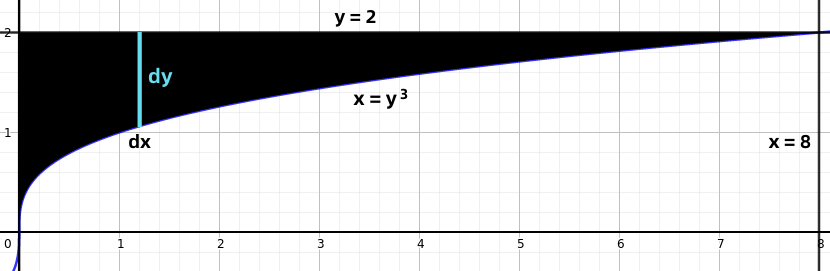
\includegraphics[width=0.65\textwidth]{"./Pictures/1dydx.png"}
		\captionof{figure}{Integrating in the order dy dx}
		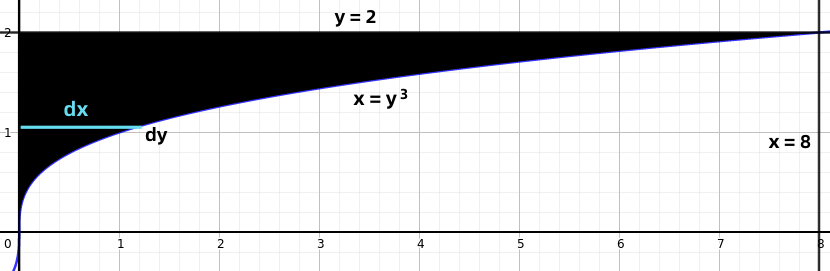
\includegraphics[width=0.65\textwidth]{"./Pictures/1dxdy.png"}
		\captionof{figure}{Integrating in the order dx dy}
	\end{center}
	$\therefore$ I = $\displaystyle \int\limits_0^2 \frac{y^3}{1+y^4} dx = \frac{1}{4} \left[\ln(|1+y^4|)\right]_0^2 = \boxed{\frac{\ln(17)}{4}}$ \\ \\ \\
	2. I = $\displaystyle \int\limits_0^2 \int\limits_{\frac{y}{2}}^1 e^{-x^2} dx \ dy = \int\limits_0^1 \int\limits_0^{2x} e^{-x^2} dy \ dx$\\ \\
	Let $u = -x^2 \implies du = -2x \ dx$ \\ \\
	$\therefore$ I = $\displaystyle -\int\limits_0^{-1}e^u du = - \left[e^u\right]_0^{-1} = \boxed{1-\frac{1}{e}}$
\end{document}